% Page 7: media and generation ER.
\subsection{媒体与生成任务的数据关系}
头像、背景和聊天立绘可以分别更换。生成图还要经过预览和确认，因此生成任务单独保存。图\ref{fig:design-er-media}中的个人媒体、当前立绘、历史归档和生成任务都归属账号。预览图只有确认后才会写入当前立绘。

\begin{figure}[H]
\centering
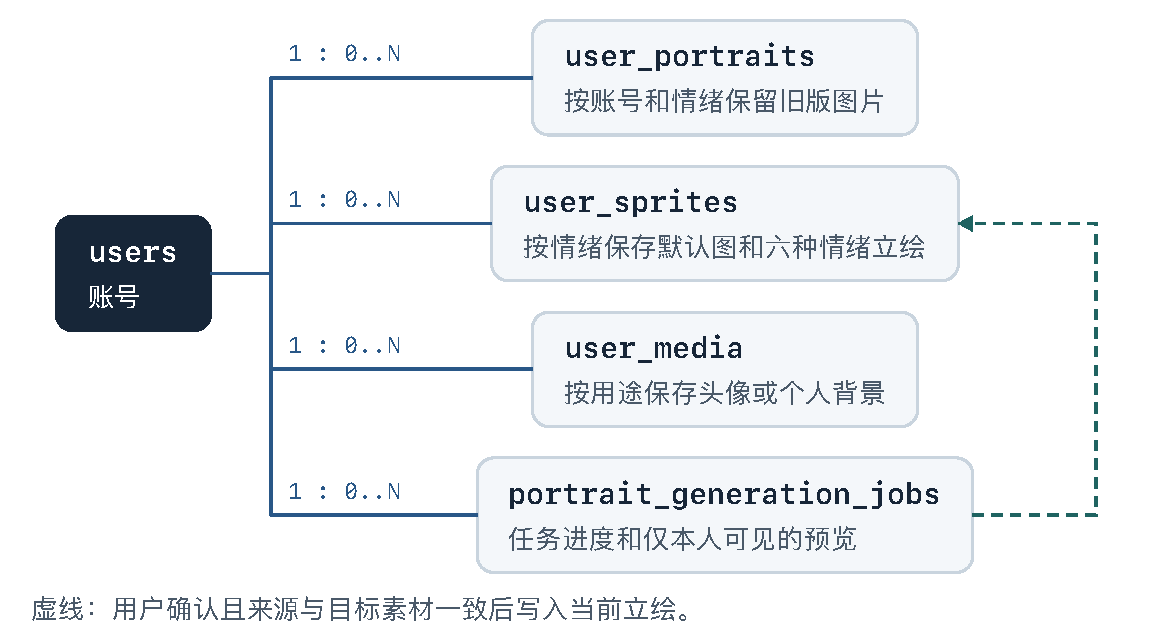
\includegraphics[width=\linewidth]{assets/design/media-er.pdf}
\caption{ER 视图二：个人媒体、历史归档与生成预览的关系}\label{fig:design-er-media}
\end{figure}

头像用于辨认用户，背景用于个人页面展示。聊天立绘按情绪分槽位，包括默认图，以及开心、难过、生气、害羞、惊讶、思考六张情绪图。替换其中一张不用重设其他图片。聊天页从当前立绘表读取对应图片。历史归档保留旧版图片，迁移时选取每个账号最新的一张旧图作为头像初始值，日常替换立绘只更新当前记录。头像、背景和立绘可分别设置。

同步时页面先取图片是否存在和更新摘要，需要展示时再读图片。背景只允许本人读取，头像和立绘可由本人查看。查看他人的资源时，当前用户须与对方有会话、待回应或已接受的纸条，或已收藏对方、持有对方的待决定卡片。纸条和消息仍按真人通信记录管理。

每个账号最多有一个生成中或待确认的任务。生成完成后先给本人看预览，再由本人确认或放弃。确认时会核对默认立绘和目标情绪图是否仍符合任务条件，通过后一起保存立绘和任务结果。素材发生变化时提示重新处理。失败、保存或放弃后清除预览。

\clearpage
